\section{¿Qué es?}

Los mapa mentales son un método efectivamente sencillo de asimilar y memoriza información a través de la representación visual de la información. 

Por naturaleza, nuestro celebro tiene un potencial ilimitado y que, en muchas ocasiones es desaprovechado o difícil de interpretar. Tenemos dos hemisferios el izquierdo y el derecho, el racional y el creativo, ambos funcionan de forma separada. Los mapas mentales consiguen relacionar ambos hemisferios (racional y creativo) y lograr que funcionen conjuntamente. 

Toda persona tiene una forma natural de elaborar sus propias ideas, mediante pensamiento irradiante\footnote{que irradia} . El pensamiento irradiante refleja mediante la asociación de ideas nuestros pensamientos y conocimientos sobre una materia concreta.  A esta forma de pensamiento podemos acceder mediante los mapas mentales, que irradian y asocian ideas a partir de un concepto central. 

\begin{figure}[htbp]
\centering
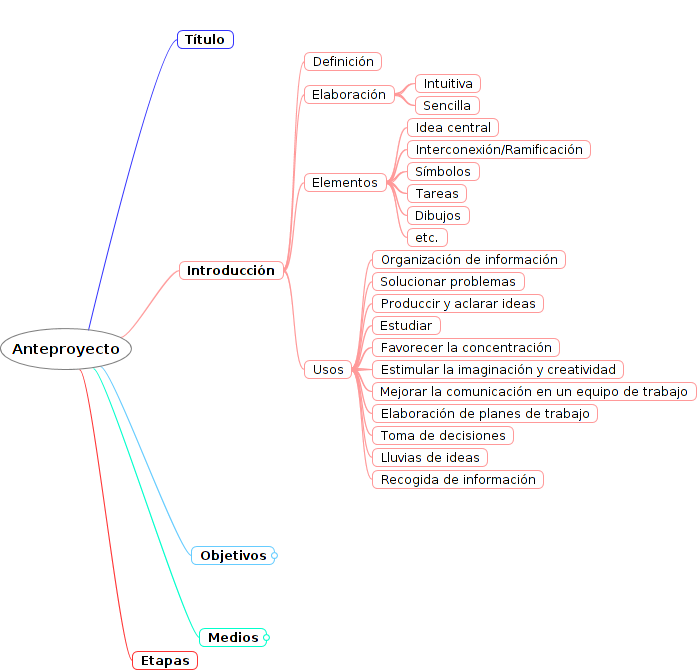
\includegraphics[width=0.9\textwidth]{imagenes/freemind}
\caption{Mapa mental de FreeMind}
\label{fig:freemind}
\end{figure}


